\documentclass{article}
\usepackage{graphicx} % Required for inserting images
\usepackage{tikz}
\usetikzlibrary{positioning,arrows}
\usetikzlibrary{arrows.meta}
\usepackage{multirow}
\title{Portfolio report}
\usepackage{pgf-pie}  
\usepackage{subcaption}
\date{\today}
\begin{document}
\maketitle
\tableofcontents      
\section*{Returns and overall performance}
\subsection*{Biggest positive and negative returns}
\begin{tikzpicture}

    \node[circle] at (0,1) {AAPL};
    
   \draw[-{Triangle[width=18pt,length=8pt]}, line width=8pt, color=green](1,0.8) -- (1, 1.4);
   \node[circle] at (0,0) {Stock with highest returns};
 
    \node[circle] at (10,1) {Burst};
    
 \draw[-{Triangle[width=18pt,length=8pt]}, line width=8pt, color=red](11,1.2) -- (11, 0.6);   
 \node[circle] at (10,-0.1) {Stock with highest negative returns};
    
    
    \node[circle] at (0,-3) {Burst};
      \draw[-{Triangle[width=18pt,length=8pt]}, line width=8pt, color=green](1,-3.2) -- (1, -2.6);
 \node[circle] at (0,-4) {Stock with highest returns in DKK};   
    
    
    \node[circle] at (10,-3) {Burst};
 \draw[-{Triangle[width=18pt,length=8pt]}, line width=8pt, color=red](11,-2.6) -- (11, -3.2);       
 \node[circle] at (10,-4) {Stock with highest negative returns in DKK};        
\end{tikzpicture}
\subsection*{}
\section*{Distribution of investments}
\subsection*{Distribution by currency and nationality}

\begin{center}


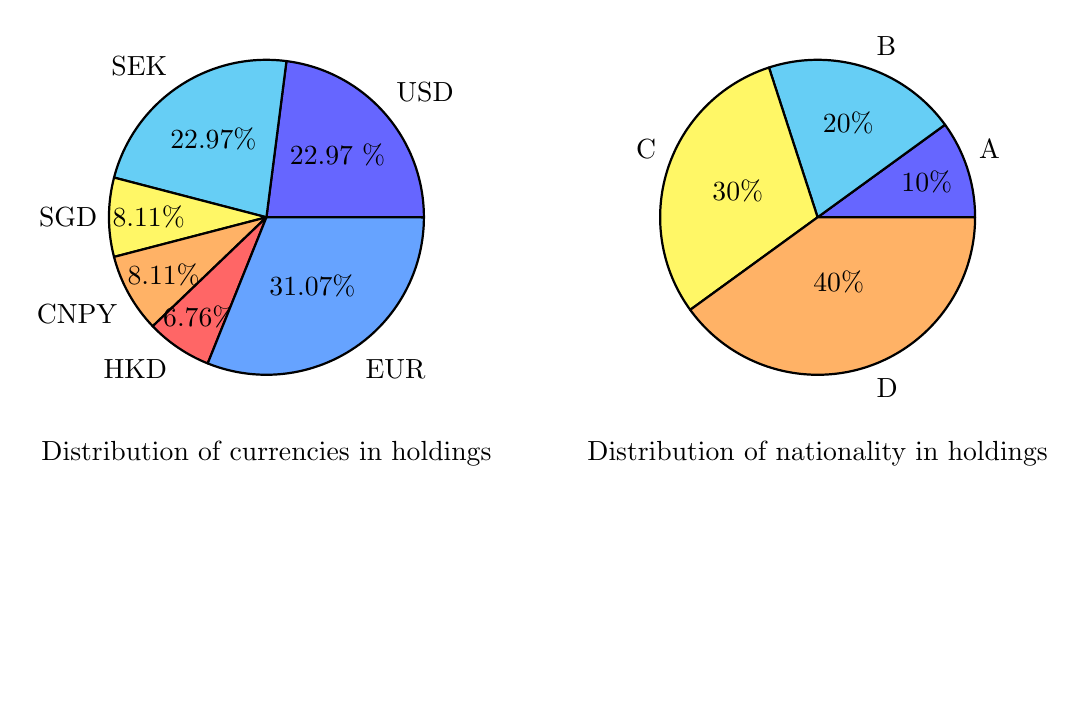
\begin{tikzpicture}[auto=left] 
\node[circle] at (-3,-3) {Distribution of currencies in holdings};
\node[circle] at (4,-3) {Distribution of nationality in holdings};
\pie[
radius=2,
pos={-3,0}
]{
	22.97 / USD,
    22.97/SEK,
    8.11/SGD,
    8.11/CNPY,
    6.76/HKD,
    31.07/EUR
    }
    
\pie[
    radius=2,
    pos={4,0},
]{10/A, 20/B, 30/C, 40/D}


\end{tikzpicture}
\end{center}
\subsection*{Distribution by sector and industry}    

\section*{Information used}
\subsection*{Conversion factors}
\begin{table}[!h]
\begin{center}
\begin{tabular}{||c ||} 
 \hline
 Col1  \\ [0.5ex] 
 \hline\hline
 1  \\ 
 \hline
 2  \\
 \hline
 3  \\
 \hline
 4  \\
 \hline
 5  \\ 
 \hline
\end{tabular}
\caption{Conversion factors for reference currency.}
\end{center}
\end{table}

\begin{table}[!h]
\begin{center}
\begin{tabular}{ |c||c|  }
 \hline
 \multicolumn{2}{|c|}{Country List} \\
 \hline
 \hline
 usd : 1   & EUR : 3\\
 EUR : 3 &   EUR : 3\\
 EUR : 3 & EUR : 3 \\
 EUR : 3   & EUR : 3\\
 EUR : 3 &   EUR : 3 \\
 EUR : 3 & \\
 EUR : 37 &\\
 \hline
\end{tabular}
\caption{Conversion factors for reference currency.}
\end{center}
\end{table}

\end{document}
